
  En esta sección veremos un caso de estudio usado para verificar la
implementación.
  El problema fue tomado de la competencia SumoUY \cite{sumouy}, el mismo
fue el desafío planteado a escolares en el año 2013.

\section {Problema}

  Se desea implementar un robot autónomo móvil que sea capaz de
hacer la entrega de un pedido en una casa determinada.
  El mismo debe moverse por un escenario e identificar las casas.
  Para recorrer la ruta de entrega, podrá valerse de una línea negra
que representará la calle de la ciudad.

  Las casas estarán ubicadas a un lado de la calle. En el recorrido
se encuentran varias casas, el robot deberá entregar un pedido
en la quinta casa por la que pase.

  El robot deberá pasar por alto las casas anteriores y
al llegar a la casa objetivo debe detenerse totalmente.

  Para probar la solución, se armará un escenario que consiste de
un piso blanco con una línea negra que puede tener curvas.

  Al lado derecho de la línea se ubicarán cajas a menos de 30
centímetros representando las casas.

\section {Solución}

  Se armó un robot móvil que cuenta con 3 sensores:

\begin{itemize}
\item Sensor de grises izquierdo
\item Sensor de grises derecho
\item Sensor de distancia apuntando hacia la derecha
\end{itemize}

  Y 2 actuadores:

\begin{itemize}
\item Motor izquierdo
\item Motor derecho 
\end{itemize}

  El robot utilizará los sensores de grises para mantenerse sobre
la línea y el sensor de distancia para saber cuándo está frente
a una casa.

  Con los motores se moverá hacia adelante inicialmente, e irá corrigiendo
  su dirección desacelerando el motor del lado que se salga de la línea.

  Durante el trayecto contará las casas, y se detendrá cuando la cuenta
llegue al valor 5.

  En el siguiente diagrama, se puede ver gráficamente de que forma
se combinan los eventos, para lograr nuestro objetivo:

\begin{figure}[hbtp]
\begin{center}
\caption{Diagrama del caso de estudio}
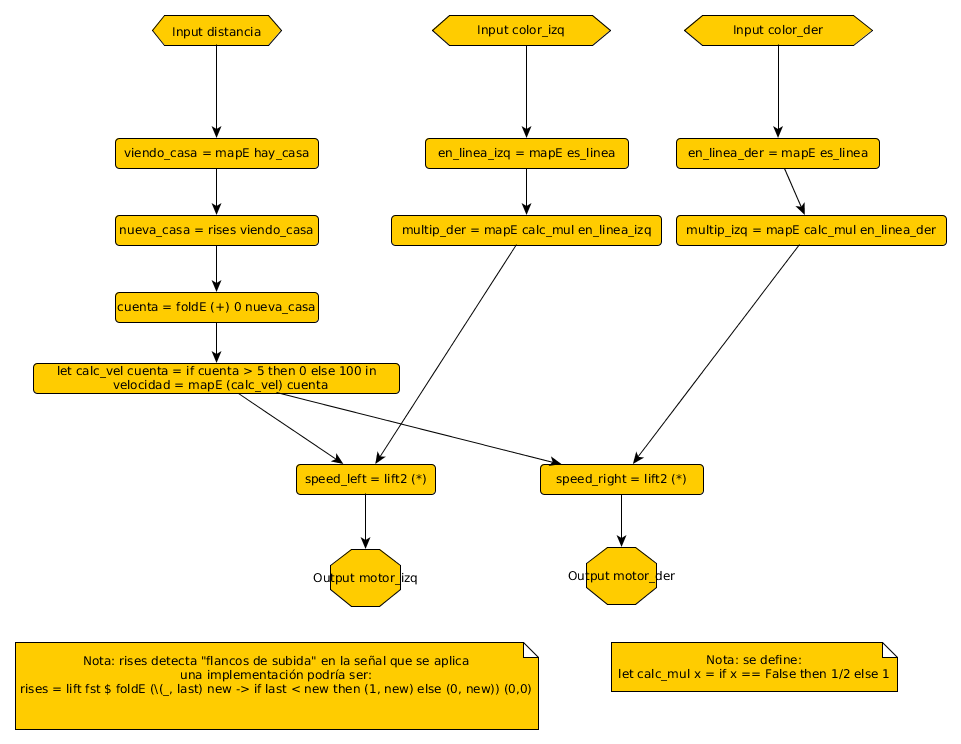
\includegraphics[width=0.9\textwidth]{graphs/delivery.png}
\label{fig:delivery}
\end{center}
\end{figure}

  Luego se llega a la implementación en el lenguaje \frob :

\begin{verbatim}

rises_last_update (_, last) new = if last < new then (1, new) else (0, new)
rises_last = foldE rises_last_update (0,0)
rises = lift fst $ rises_last
accumulate = foldE (+) 0

hay_casa d = if (d < MIN) then 1 else 0
velocidad_casa num = if (num >= 5) then 0 else 100

es_linea gris = gris > MIN_NEGRO
calc_mul linea = if (linea == False) then 1/2 else 1

main = do {
         distance <- read INPUT_DISTANCE
         color_izq <- read INPUT_DISTANCE
         color_der <- read INPUT_DISTANCE

         viendo_casa <- lift hay_casa distance,
         nueva_casa <- rises viendo_casa,
         cuenta <- accumulate nueva_casa,
         velocidad <- lift velocidad_casa cuenta,

         en_linea_izq <- lift es_linea color_izq,
         en_linea_der <- lift es_linea color_der,
         multip_izq <- lift calc_mul en_linea_der,
         multip_der <- lift calc_mul en_linea_izq,

         speed_left <- lift2 (*) (velocidad multip_izq)
         speed_right <- lift2 (*) (velocidad multip_der)

         output MOTOR_IZQ <- speed_left
         output MOTOR_DER <- speed_right
       }

\end{verbatim}

\section {Conclusiones del caso}


